\documentclass[xcolor=dvipsnames,usepdftitle=false]{beamer} 
%\usecolortheme[named=BlueViolet]{structure} 
\usecolortheme[RGB={83,13,88}]{structure} \usetheme[height=7mm]{Boadilla} 
\setbeamertemplate{items}[ball] 
\setbeamertemplate{navigation symbols}{}%remove navigation symbols 

\usefonttheme[onlylarge]{structuresmallcapsserif}
\usefonttheme{professionalfonts}

% Normal usepackage includes
\usepackage{graphicx}
\usepackage{color}
\usepackage{amsfonts}
\usepackage{amssymb}
\usepackage{textcomp}
\usepackage{amsthm}
\usepackage{amsopn}
\usepackage{subfigure}
\usepackage{fancybox}
\usepackage{mathtools}
%Set up command for logo in top right corner
\usepackage[absolute,overlay]{textpos}
\setlength{\TPHorizModule}{1mm}
\setlength{\TPVertModule}{1mm}
\newcommand{\MyLogo}{%
	\begin{textblock}{14}(119.0,1.0) %logo position
		
\includegraphics[width=0.8cm]{pictures/logo_only.eps}
	\end{textblock}
}

% This puts in a section ``title slide'' when \section command
% is encountered.  Can easily be changed to subsection
\AtBeginSection{
\begin{frame}
		\MyLogo
\begin{center}
		\structure{\Large \insertsection}
	\end{center}
\end{frame}
}

%Use some script greek letters
\renewcommand\epsilon{\varepsilon}
\renewcommand\phi{\varphi}
\renewcommand\theta{\vartheta}

%Macros for standard sets
\newcommand{\newVar}[2]{\newcommand{#1}{\ensuremath{#2}\xspace}}
\newVar\Naturals{\mathbb{N}}
\newVar\Integers{\mathbb{Z}}
\newVar\Rationals{\mathbb{Q}}
\newVar\Reals{\mathbb{R}}
\newVar\Complex{\mathbb{C}}

%++++++++++++++++++++++++++++++++++++++++++++++++++++++++++++++++++++++++++++++++++++++++++++++++++%
%Macros for math functions that take an argument
\newcommand{\ldb}{\text{\textlbrackdbl}}
\newcommand{\rdb}{\text{\textrbrackdbl}}

\newcommand{\norm}[1]{\ensuremath{\lVert#1\rVert}}
\newcommand{\abs}[1]{\ensuremath{\lvert#1\rvert}}
\newcommand{\ceil}[1]{\ensuremath{\lceil#1\rceil}}
\newcommand{\floor}[1]{\ensuremath{\lfloor#1\rfloor}}
\newcommand{\set}[1]{\ensuremath{\{#1\}}}
\newcommand{\angular}[1]{\ensuremath{\langle#1\rangle}}
\newcommand{\paren}[1]{\ensuremath{(#1)}}
\newcommand{\sset}[1]{ \{ #1 \} }
\newcommand{\dset}[2]{ \{ #1 \mid #2 \} }

\newcommand{\Norm}[1]{\ensuremath{\left\lVert#1\right\rVert}}
\newcommand{\Abs}[1]{\ensuremath{\left\lvert#1\right\rvert}}
\newcommand{\Ceil}[1]{\ensuremath{\left\lceil#1\right\rceil}}
\newcommand{\Floor}[1]{\ensuremath{\left\lfloor#1\right\rfloor}}
\newcommand{\Set}[1]{\ensuremath{\left\{#1\right\}}}
\newcommand{\Angular}[1]{\ensuremath{\left\langle#1\right\rangle}}
\newcommand{\Paren}[1]{\ensuremath{\left(#1\right)}}
\newcommand{\Ssett}[1]{ \{ #1 \} }
\newcommand{\Dset}[2]{ \{ #1 \mid #2 \} }

\newcommand{\Average}[1]{\ensuremath{\{ \! \! \{ #1 \} \! \! \}} }
\newcommand{\Jump}[1]{\ensuremath{\ldb #1 \rdb}}
\newcommand{\average}[1]{\ensuremath{\{ \! \! \{ #1 \} \! \! \}} }
\newcommand{\jump}[1]{\ensuremath{\ldb #1 \rdb}}
\newcommand{\diam}[1]{\ensuremath{ \mathrm{diam}(#1) }}

\newcommand\st{\;|\;}


\begin{document}

\title{Relativity and the Global Positioning System}
\author{James Fielder}
\institute{Durham University}
\date{Feburary 13$^\text{th}$ 2013}

\begin{frame}[plane]

\titlepage

\end{frame}

\begin{frame}

\frametitle{Intro}

Relativity plays a large part in how the global positioning system works. Both in the fundamental method as to how the system works, and in calculating errors to both earth bound and satellite clocks.

\end{frame}

\begin{frame}

\frametitle{Contents}

\begin{itemize}
	\item Fundamental operation of GPS
	\item Main relativistic errors in GPS
	\item The Sagnac effect
\end{itemize}

\end{frame}

\begin{frame}

\frametitle{Fundamentals of GPS}

GPS works by solving the following equation for time $t$ and position $\vec{r}$ variables: \[ c^2 (t-t_i)^2 = |\vec{r}-\vec{r}_i|^2 \] 
given signals from 4 GPS satellites. 

\vspace{\baselineskip}

This relies on the fundamental postulate of special relativity: that the speed of light is the same in all inertial frames.

\end{frame}

\begin{frame}

\frametitle{Fundamentals of GPS}

\begin{center}

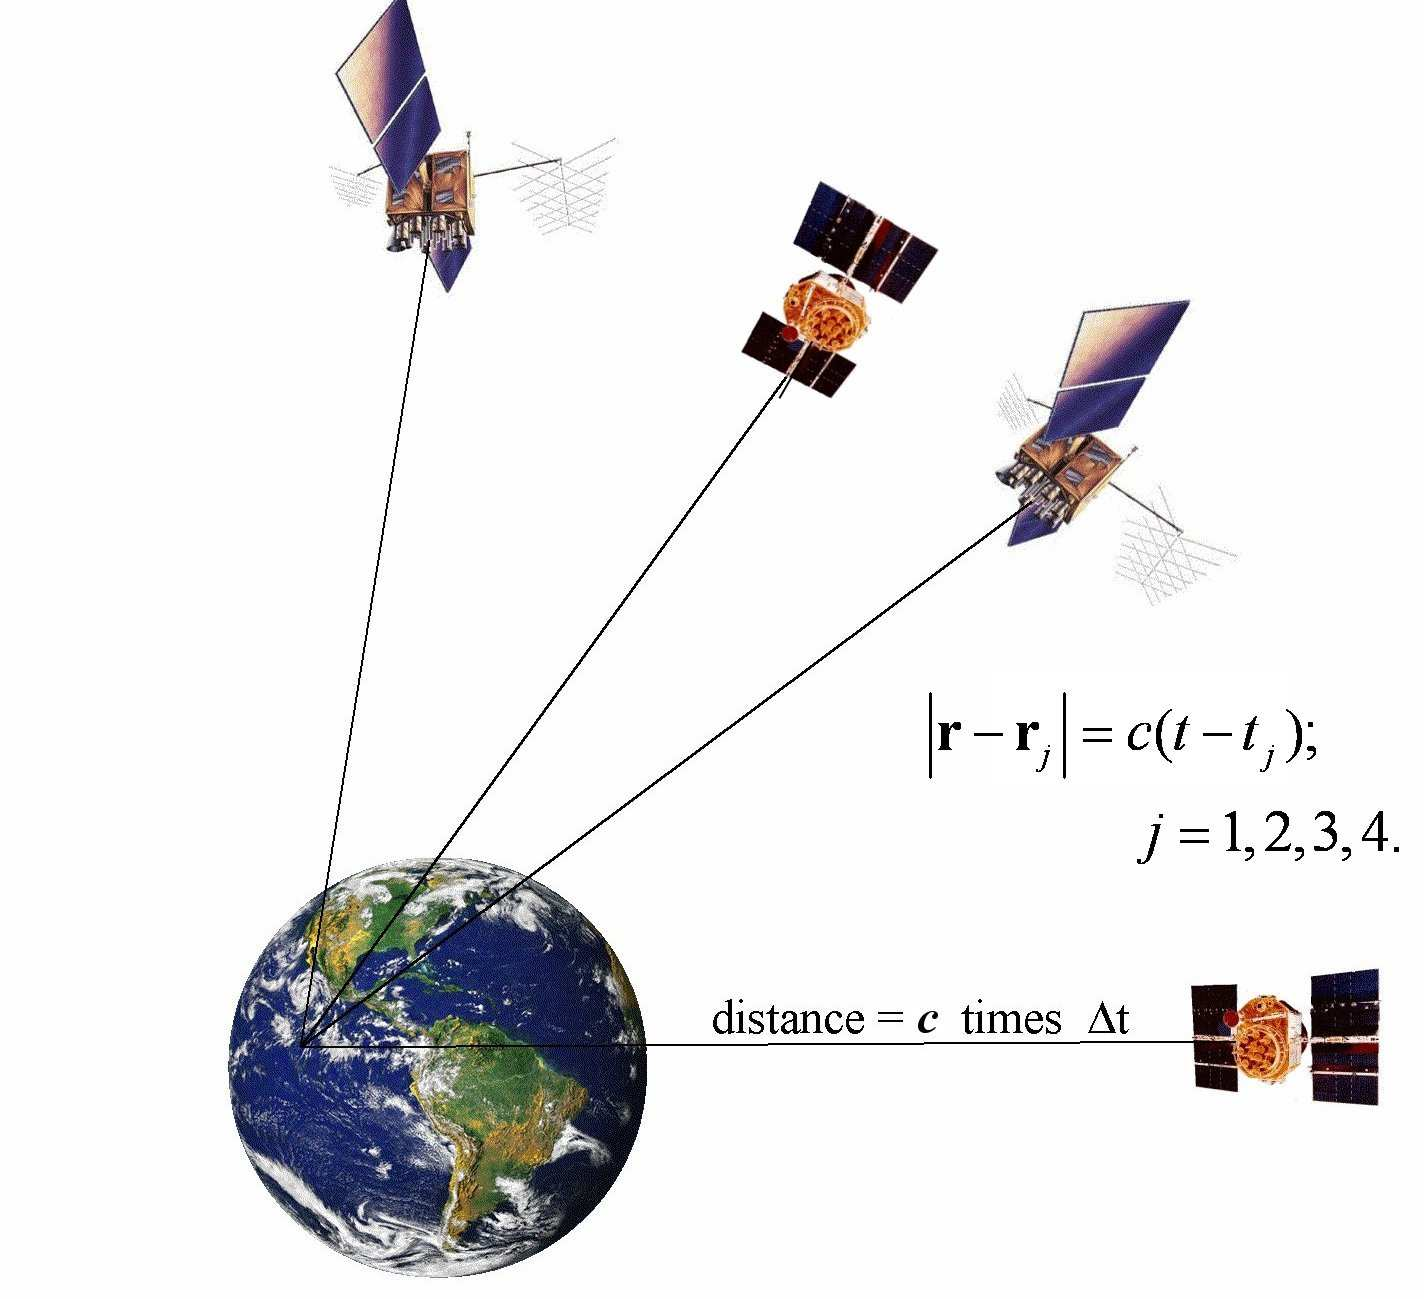
\includegraphics[scale=0.18]{images/eqn.png}

\end{center}

\end{frame}

\begin{frame}

\frametitle{Relativistic errors in GPS}

\begin{itemize}
	\item Time dilation due to the motion of the satellites
	\item Gravitational time dilation due to the earth's gravitational field
	\item The Sagnac effect
	\item Doppler shifts in radio frequencies
\end{itemize}

\end{frame}

\begin{frame}

\frametitle{The Sagnac effect}

The Sagnac effect is caused by the rotation of the earth. We have to correct for that fact that a satellite ahead of the rotation of the earth will receive a signal before a signal from a satellite which is behind the rotation of the earth.

Recall the Minkowski line element from special relativity in cylindrical coordinates: \[ -ds^2 = -(c dt)^2 + dr^2 + r^2 d\phi^2 + dz^2 \]

We now transform this into a new spacetime where the azimuthal coordinate rotates with constant speed $\omega_{e}$.

\[ t = t' , \,\,\,\,\,\, r=r', \,\,\,\,\,\, \phi = \phi' + \omega_{e} t', \,\,\,\,\,\, z = z' \]

\end{frame}

\begin{frame}

\frametitle{The Sagnac effect}

This gives us a line element for a rotating frame in flat space:

\[-ds^2 = - \left(1- \frac{\omega_{e}^2 {r'}^2}{c^2}\right)(cdt')^2 + 2 \omega_{e} {r'}^2 d\phi' dt' + (d\sigma)^2\]

\vspace{\baselineskip}

with $(d\sigma)^2 = (dr')^2 + (r' d \phi)^2 + (dz')^2$

\end{frame}

\begin{frame}

\frametitle{The Sagnac effect}

This gives us a line element for a rotating frame in flat space:

\[-ds^2 = - \underbrace{\left(1- \frac{\omega_{e}^2 {r'}^2}{c^2}\right)(cdt')^2 + 2 \omega_{e} {r'}^2 d\phi' dt'}_{\text{Time dependent}} + \overbrace{(d\sigma^2)}^{\mathclap{\text{Time Independent}}}\]

\vspace{\baselineskip}

with $(d\sigma)^2 = (dr')^2 + (r' d \phi')^2 + (dz')^2$ 

\vspace{\baselineskip}

We need to find the time that light takes to travel in this coordinate system. Remember that $ds^2 = 0$ for light rays. Also note that $\frac{\omega_{e}^2 {r'}^2}{c^2}$ is very close to zero. We now form an equation for $(cdt')^2$

\end{frame}

\begin{frame}

\frametitle{The Sagnac effect}

\[(cdt')^2 - \frac{2\omega_{e} {r'}^2 d\phi' (cdt')}{c} - (d \sigma)^2 = 0 \]

This gives:

\[c dt' = d\sigma + \frac{\omega_{e} {r'}^2 d\phi'}{c}\]

\vspace{\baselineskip}

We can now integrate over the path to find the time of travel. 

\[\int_{path} dt' = \int_{path} \frac{d \sigma'}{c} + \frac{2\omega_{e}}{c^2} \int_{path} d {A'}_{z} \]

where $A_z$ is a projection from the path along the surface to an area on a plane through the equator.
\end{frame}

\begin{frame}

\frametitle{The Sagnac effect}

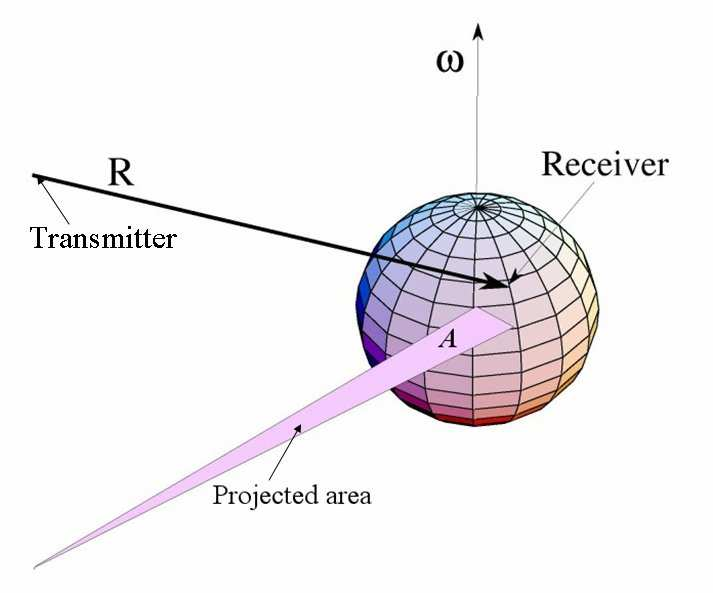
\includegraphics[scale=0.4]{images/sagnac.png}

\end{frame}

\begin{frame}

\frametitle{Overall difference due to the Sagnac effect}

\begin{itemize}
	\item The Sagnac effect depends on how close to the equator you are. \vspace{\baselineskip}
	\item At the equator this means a discrepancy of up to $\pm 207 ns$ in the time that signals from the GPS satellites take to reach a receiver.
\end{itemize}

\end{frame}

\begin{frame}

\frametitle{Conclusions}

Relativity plays a very large part in our understanding and implementation of the GPS system. Without Einstein's revolutionary ideas about space and time the system could not function properly.

\vspace{\baselineskip}

GPS is used by millions devices daily to guide them around on the earth, all of which work flawlessly. What excellent evidence that Einstein's theores are completely correct.

\end{frame}

\begin{frame}[plain]

\begin{center}
Any questions?
\end{center}

\vspace{\baselineskip}

\textbf{Further Reading} 

Relativity, Gravitation and Cosmology - Ta-Pei Cheng 

\vspace{\baselineskip}

Gravity: An introduction to Einstein's Relativity - James B. Hartle 

\vspace{\baselineskip}

Relativity in the Global Positioning System - Neil Ashby - http://www.livingreviews.org/lrr-2003-1 

\vspace{\baselineskip}

Global Positioning System: Theory and Applications Vol 1 - Neil Ashby and James Spilker - pages 623 - 697 
\end{frame}

\end{document}